\documentclass[11pt]{amsart}
%\documentclass[11pt,a4paper]{amsart}

% use up more of the page
\addtolength{\topmargin}{-5mm}
\addtolength{\textheight}{15mm}
\addtolength{\oddsidemargin}{-11mm}
\addtolength{\evensidemargin}{-11mm}
\addtolength{\textwidth}{25mm}

\renewcommand{\baselinestretch}{1.05}

\usepackage{amsmath,amssymb,xspace}
\usepackage{natbib}
\usepackage{verbatim,fancyvrb}
\usepackage[final]{graphicx}

% hyperref should be the last package we load
\usepackage[pdftex,
                colorlinks=true,
                plainpages=false, % only if colorlinks=true
                linkcolor=blue,   % only if colorlinks=true
                citecolor=black,   % only if colorlinks=true
                urlcolor=magenta     % only if colorlinks=true
]{hyperref}

\newcommand{\eps}{\epsilon}

\newcommand{\RR}{\mathbb{R}}

\newcommand{\Hij}{H_{i,j}}
\newcommand{\Pij}{P_{i,j}}
\newcommand{\psiij}{\psi_{i,j}}
\newcommand{\Wlij}{W^l_{i,j}}
\newcommand{\Wij}{W_{i,j}}
\newcommand{\Yij}{Y_{i,j}}

\newcommand{\bF}{\mathbf{F}}
\newcommand{\bQ}{\mathbf{Q}}
\newcommand{\bW}{\mathbf{W}}

\newcommand{\bn}{\mathbf{n}}
\newcommand{\bq}{\mathbf{q}}
\newcommand{\bs}{\mathbf{s}}
\newcommand{\bv}{\mathbf{v}}

\newcommand{\hpw}{\hat P}
\newcommand{\Cavit}{C_{avit}}
\newcommand{\Cmelt}{C_{melt}}
\newcommand{\Creep}{C_{reep}}



\title[PISM hydrology model]{A subglacial hydrology model \\for the Parallel Ice Sheet Model (PISM)}

\author[van Pelt and Bueler]{Ward van Pelt and Ed Bueler}


\begin{document}

\maketitle

\begin{quote}
\textbf{Abstract}:  \emph{The hydrology model we propose for PISM is inspired by  \emph{\citet{Schoofmeltsupply,Schoofetal2012,Hewitt2011,Hewittetal2012}}.  The mass of water is conserved.  The transport of water is driven by the pressure gradient; the flow is Darcian.  An elliptic equation determines water pressure from physical models for aquifer opening (wall melt, sliding) and and closure (creep) processes.  The pressure equation arises by comparing two evolution equations for water amount.  A conduit (channel) network is not, however, modeled.  We numerically approximate by an implicit finite difference method.  The nonlinear algebraic equations for each time-step of this  scheme are solved by parallel Newton iterations.  We address verification of the numerical scheme, the degree to which the model scales to large ice sheets, and parameter identification using GPS data.}
\end{quote}

\thispagestyle{empty}

\setcounter{tocdepth}{1}
\tableofcontents

\section{Introduction}

Our goal is to capture the major qualities of an evolving drainage system, without over-specifying a particular system morphology.  We want to limit the number of unknown parameters.  The qualities captured by our model are:
\renewcommand{\labelenumi}{\emph{(\roman{enumi})}\quad}
\begin{itemize}
\item liquid water lives in a sheet-like system,
\item its mass is conserved,
\item water flows from high to low hydraulic potential,
\item the capacity of the drainage system evolves according to physical opening and closing processes,
\item water pressure is bounded above by overburden pressure,
\item we do not use a local function relating water pressure to water amount \citep[c.f.][]{FlowersClarke2002_theory}, and
\item the yield stress of the subglacial layer, which determines the basal shear stress under the ice sheet, depends on the water pressure.
\end{itemize}
We will connect this hydrology model to ice dynamics in a flexible and generic manner that can be applied by PISM users to ice sheets and glaciers.


\section{Elements of a subglacial aquifer model}

\subsection*{Conserved subglacial water in a sheet-like layer}
The evolution of the water thickness $W(t,x,y)\ge 0$ is described by the mass conservation equation,
\begin{equation} \label{eq:conserve}
\frac{\partial W}{\partial t} + \nabla \cdot \bQ = \Phi \, ,
\end{equation}
where $\bQ$ is the water flux, with SI units $\text{m}^2\,\text{s}^{-1}$, and $\Phi$ is a source term.  We will be able to construct, in later sections, numerical schemes for equation \eqref{eq:conserve} which display discrete conservation even if $\bQ$ and $\Phi$ represent highly-irregular and/or highly-parameterized functions.  We write the water sources
\begin{equation} \label{eq:watersources}
  \Phi = \rho_w^{-1} \left(m + S\right)
\end{equation}
where $\rho_w$ is the density of fresh liquid water, $m$ is the rate at which basal melting (refreeze) of ice adds (removes) water, and $S$ is the rate at which surface runoff or englacial drainage adds water.  Groundwater could also contribute to the aquifer \citep[e.g.][]{DeFooretal2011}, and this would be included in $\Phi$, but we do not attempt to model it here.  Note $m$ and $S$ have units $\text{kg}\,\text{m}^{-2}\,\text{s}^{-1}$ while $\Phi$ has units $\text{m}\,\text{s}^{-1}$.

In applications $m$ and $S$ are coupling terms to other components of the ice flow model, but here we regard $\Phi=\Phi(t,x,y)$ as a known function.  Basal melt $m$ is a function of the conservation of energy model \citep{AschwandenBuelerKhroulevBlatter}, while surface drainage $S$ is related to ice geometry and surface mass/energy processes \citep[e.g.][]{vanPeltetal}.  We will return to the parameterization of melt below.

The layer thickness $W$ here is only meaningful if it is regarded as an average over a horizontal scale of tens to thousands of meters.  In fact, because the numerical schemes used to discretize this model have horizontal cell sizes of $100$ m to $10$ km, process models for the evolution of channels, the geometry of cavities, the transport of sediment, the penetration of ice into the mineral base, and many other details of aquifer morphology are, of necessity, beyond the scope of this article.  We will attempt only to model spatially-averaged versions of water amount and water pressure.

\subsection*{Darcian flux}  We relate the water flux $\bQ$ in \eqref{eq:conserve} to the gradient of the hydraulic potential $\psi$ \citep{Clarke05, FlowersClarke2002_theory}:
\begin{equation}
\bQ = - \frac{K \, W}{\rho_w g} \nabla \psi
\label{eq:flux}
\end{equation}
Here, $\rho_w$ is the water density, $g$ the gravitational acceleration and $K$ the effective hydraulic conductivity.  Conductivity $K$ combines with the aquifer thickness to determine the transmissivity of the system \citep{PimentelFlowersSchoof2010}.  By \eqref{eq:flux}, water flows from high to low fluid potential.  By definition, $\psi$ combines the water pressure $P(t,x,y)$ and the gravitational potential,
\begin{equation} \label{eq:potential}
\psi = P + \rho_w g\, b,
\end{equation}
where $z=b(x,y)$ is the bedrock elevation.  From equations \eqref{eq:flux} and \eqref{eq:potential}, flow depends on both horizontal gradients in the water pressure and on the bedrock slope.  Because the bedrock elevation comes from rough data, in practice, and also because the pressure $P$ will be subject to inequalities (below), the reader should suppose that the hydraulic potential is minimally smooth.  The gradient $\nabla \psi$ will be seen to have significant spatial variability in practice.


\subsection*{Implicitly-determined water pressure}  Subglacial water pressure is always related in some manner to the downward normal stress from the ice, the overburden stress.  We choose a particular form for the overburden stress, the standard hydrostatic approximation for the ice \citep{Clarke05}.  First we identify the normal stress with the ice pressure $P_o$ (overburden ``pressure'').  Then we use a shallow approximation \citep{Fowler} to compute it:
\begin{equation}\label{eq:shallowoverburden}
  P_o = \rho_i g H.
\end{equation}
Here $H(t,x,y)$ is the ice thickness and $\rho_i$ is the density of the ice.   This is an adequate approximation because, in part, the equations in the next section for aquifer evolution are sufficiently uncertain so that the modelling errors made by using \eqref{eq:shallowoverburden} are likely to be a modest portion of the total error.

Mathematical closure might suggest that water pressure $P$ is a point-wise (local) function of the water amount $W$.  For example, \citet[equation (30)]{FlowersClarke2002_theory} choose a power law $P = P_o (W/W_{crit})^\sigma$ where $W_{crit}>0$ is a constant critical water thickness and $\sigma>1$ is a constant.  Note that if the drainage system is locally-filled, i.e.~if $W=W_{crit}$, then the water pressure equals the ice overburden pressure $P_o$, but by this model $P$ can exceed $P_o$.  Models using such a local function are essentially forms of the porous medium equation \citep{VazquezPME}.  Such models do not capture the observation that the hydrological system can become pressurized or depressurized by distant, non-local changes in water amount [REF].   Models using this closure have, however, been applied to the Vatnaj\"okull ice cap by \citet{Flowersetal2005}, and were extended to include more complete stress balance in \citet{PimentelFlowersSchoof2010} and \citet{PimentelFlowers2011}.

The expression for $P$ currently used in PISM is also such a local closure.  It is the simpler rule $P = \alpha P_o W/W_0$, where $W$ is a not-conserved water thickness, $\alpha$ is a constant, typically $0.9\le \alpha < 1$, and $W_0=2$ m is a fixed capacity parameter \citep[equation (20)]{BBssasliding}.

As in \cite{Schoofetal2012,Hewittetal2012} we apply bounds to $P$.  Specifically, in our model $P$ does not exceed the overburden pressure:
\begin{equation} \label{eq:pressurebounds}
0 \le P \le P_o.
\end{equation}
This simplification omits possibly-significant ``uplift'' scenarios which occur on short timescales [REF].  We regard such events as beyond the scope of large-scale ice sheet modelling.

We will in all cases determine an equation for $P$ by equating two distinct concepts for the evolution of water thickness, first conservation of water and second evolution of aquifer capacity.  As a result, the pressure is determined implicitly by an equation that is (generally) an elliptic PDE.  This equation applies at each time $t$ to the entire region where $W>0$, and it determines $P$ from boundary conditions.

FIXME:  or we could do something simple for part of the water flow by assuming $P=P_i$ \citep{LeBrocqetal2009}

\subsection*{Evolution of aquifer capacity}  Our hydrology model conserves water (equation \eqref{eq:conserve}) and also evolves aquifer capacity (equation \eqref{eq:capacityevolution} below).  The latter evolution equation includes physical opening and closure processes.

Subglacial aquifers are highly-dynamic systems and generally no single variable controls efficiency \citep[e.g.][]{Bartholomausetal2008}, but a drainage system can operate in at least two modes, a faster channelized mode and a slower distributed mode which may have the morphology of linked cavities \citep{Schoofmeltsupply}.  The subglacial drainage system opens because of glacier sliding and because moving water in the aquifer causes wall (ceiling) melt of the ice.  Glacier sliding also opens cavities.  On the other hand,  the downward creep of the ice tends to close the system \citep{Hewitt2011,Walder1982}.

We believe a sheet-like approach to system capacity can combine these major qualities of both linked-cavity systems and channeled flow, but we will not individually model either cavity or channel features.  Only in an area-averaged sense can we model the wall melt of individual conduits, the creation of cavities by sliding, and the closure of conduits and cavities by creep.  Our continuum model can only describe the evolution of averages over many multiples of the width scale of these features.

A stable sheet-like subglacial aquifer requires poorly-sorted till and bed protrusions to possess stable sheet-like states \citep{CreytsSchoof2009}.  Without such bed protrusions instabilities disallow significant sheet-like drainage \citep{Walder1982}.  We assume that the till properties needed to justify the use of a stable sheet-like model apply at all locations under the glacier or ice sheet.

The sheet-like aquifer has a thickness $Y$ which evolves by a differential equation which has terms for opening by wall (ceiling) melting, opening by cavitation from sliding, and closure as a function of the creep of the ceiling and walls of conduits, sheets, and cavities.  Our proposed equation is similar to equation (1) in \citet{Schoofmeltsupply}, and it is an instance of equation (10) in \citet{Hewitt2011}:
\begin{equation} \label{eq:capacityevolution}
\frac{\partial Y}{\partial t} = \frac{m}{\rho_i} + \Cavit |\bv_b| - \Creep A (P_o - P)^n W.
\end{equation}
The terms on the right side of \eqref{eq:capacityevolution} represent wall melt, cavitation, and creep closure, respectively.  Here $m$ is again the mass-per-area rate of wall melt of the ice, $\bv_b$ is the sliding velocity, $A$ is the ice softness in Glen's law \citep{Paterson}, $n$ is Glen's exponent for ice deformation, the difference $P_o-P$ is the effective pressure, and $\Cavit,\Creep$ are dimensionless positive constants.  Because of \eqref{eq:pressurebounds}, the effective pressure is positive ($P_o \ge P$) so the creep term is always either a closure term or it is inactive when the water pressure is at overburden.  The creep closure term is proportional to the water thickness $W$ based on the concept that, as water accumulates in the sheet, the ice will reduce its contact area with the bedrock, leading to enhanced downward motion of the conduit/cavity roof at the same effective pressure \citep{Hewitt2011}.


\subsection*{Wall melt}  The wall melt $m$, which appears in equations \eqref{eq:watersources} and \eqref{eq:capacityevolution}, is determined by energy balance \citep{Hewitt2011}.  Friction from sliding, geothermal flux, conduction into the ice above, dependence of the melting point on pressure, and the rate at which the kinetic energy of the water is dissipated all contribute to the wall melt rate.  In fact, a relatively-complete description in terms of the enthalpy $E$ of the basal ice \citep{AschwandenBuelerKhroulevBlatter} and the enthalpy $E_l(P)$ of the subglacial water is
\begin{equation}\label{eq:meltmaximal}
(E_l(P) - E)\, m = -\vec \tau_b\cdot \bv_b + q_{lith} - q_{ice} - \rho_w W \frac{\partial E_l(P)}{\partial P} \frac{dP}{dt} - \Cmelt \mathbf{Q} \cdot \nabla \psi.
\end{equation}
Here $\vec\tau_b$ is the basal shear stress, $q_{lith}$ is the upward (lithospheric) geothermal flux, $q_{ice}$ is the heat flux upward into the ice, and $dP/dt$ is the material derivative following the water flow.  Equation \eqref{eq:meltmaximal} follows from equation (50) in \citet{AschwandenBuelerKhroulevBlatter}, with added dissipation term ``$- \Cmelt \mathbf{Q} \cdot \nabla \psi$''.  Because of the uncertainties in parameterization \eqref{eq:flux} for water flux, we add the tunable coefficient $0\le \Cmelt \le 1$ to the expression.

If the temperature $T$ of the base of the ice is colder than the pressure melting temperature $T_m(P)$ of the water, and if the heat capacity of ice is assumed to have a temperature-independent value $c_i$, then the coefficient on the left side of \eqref{eq:meltmaximal} satisfies
	$$E_l(P) - E = L + c_i (T_m(P) - T)$$
where $L$ is the latent heat of fusion \citep[equations (4) and (8)]{AschwandenBuelerKhroulevBlatter}.  If, on the other hand, the basal ice is temperate, so it is at the pressure-melting temperature and has a liquid water fraction $0\le \omega < 1$, then
	$$E_l(P) - E = (1-\omega) L + c_i (T_m(P) - T_m(P_o)).$$

Thus a simplified form of \eqref{eq:meltmaximal} would use $E_l(P) - E \approx L$ on the assumptions that the basal ice is always close to the pressure melting temperature ($T\approx T_m(P) \approx T_m(P_o)$) and that the liquid water fraction of temperate ice is small ($\omega \approx 0$).  In fact, Equation \eqref{eq:meltmaximal} extends the standard parameterization of melt represented by equation (12) in \citet{Hewitt2011}.  If we make the already-mentioned simplifications, and if we also assume that the variation of the enthalpy of the water with pressure is insignificant ($\partial E_l(P)/\partial P \approx 0$), and denoting $G=q_{lith} - q_{ice}$, then \eqref{eq:meltmaximal} reduces to the equation in \citet{Hewitt2011},
\begin{equation}\label{eq:melthewitt}
L\, m = -\vec \tau_b\cdot \bv_b + G - \Cmelt \mathbf{Q} \cdot \nabla \psi.
\end{equation}
We will use equation \eqref{eq:melthewitt} here for simplicity.  However, consistency of the current hydrology submodel with the rest of PISM suggests returning to equation \eqref{eq:meltmaximal} for more complete conservation of energy when determining the basal melt rate \citep{AschwandenBuelerKhroulevBlatter}.


\subsection*{Plastic till}  Our model for water flow in the subglacial aquifer could allow the water amount $W$ to evolve without influencing the macroscopic ice flow.  However, a primary interest is in the connection of hydrology to glacier dynamics.  The most significant connection is that the strength of the subglacial layer depends on the water pressure $P$.  In fact, we propose to use a Mohr-Coulomb or ``plastic'' relation for the yield stress \citep{Clarke05, SchoofStream, SchoofTill}, and such a relation is already in  use in PISM \citep{BBssasliding,Winkelmannetal2011}.  In this relation the effective pressure $P_o - P$, which the ice applies to the till layer, is one factor, while the other factor is a till-friction angle $\phi$ which may vary over the ice sheet \citep{BBssasliding}.  Generally we may add a small positive till cohesion $c_0$:
\begin{equation} \label{eq:mohr-coulomb}
  \tau_c = c_0 + (\tan{\phi}) (P_o - P).
\end{equation}
Spatial variations in the till-friction angle $\phi$ may be used to model the marine history of sediments \citep[e.g.][]{Martinetal2011}.  Temporal evolution of $\phi$ could also arise from sediment transport.

Using \eqref{eq:mohr-coulomb}, the simplest membrane-stress-balancing ice dynamics model, which is the shallow shelf approximation \citep{WeisGreveHutter}, applies to both floating and grounded ice in a well-posed way, resulting in ice sheets which contain ice streams  \citep{SchoofStream}.  This stress balance is in current use in PISM \citep{BBssasliding}.  It remains well-posed when $\tau_c=0$ over large areas, including ice shelves, as long as total basal shear stress under the ice sheet suffices to keep the whole ice mass from sliding into the ocean \citep{SchoofStream}.  Regions with $\tau_c=0$ do not represent a particular difficulty, at a mathematical or numerical level, if membrane stresses can balance the distributed driving stresses by connecting each part of the ice sheet/shelf system to sufficient basal resistance.

The pseudo-plastic power-laws also allowed in PISM \citep{pism-user-manual} have a (pseudo) yield stress coefficient also denoted ``$\tau_c$'', and these laws also use equation \eqref{eq:mohr-coulomb}.  It is reasonable to suppose that near-plastic power laws generate flows which are close to those for the plastic relation itself \citep{SchoofCoulombBlatter}.


\section{Solvable mathematical models}

\subsection*{Alternatives} The hydrology model in this paper is based on the elements already given.  Specifically these are the positivity of water thickness ($W\ge 0$), the pressure inequalities \eqref{eq:pressurebounds}, and the seven equations \eqref{eq:conserve}, \eqref{eq:watersources}, \eqref{eq:flux}, \eqref{eq:potential}, \eqref{eq:shallowoverburden}, \eqref{eq:capacityevolution}, and \eqref{eq:melthewitt}.

Distinct mathematical models arise from added assumptions about the relationship between water thickness $W$ and the capacity thickness $Y$, on the one hand, and about the nature of hydraulic conductivity $K$, on the other.  These assumptions are necessary to ``close'' the model and give a uniquely-solvable mathematical problem.

Here are some possibilities for the relationship between $W$ and $Y$:
\renewcommand{\labelenumi}{\Alph{enumi}.}
\begin{enumerate}
\item The water is assumed to fill the subglacial cavity in all cases, so $W=Y$.
\item FIXME: as in Hewitt et al poster at AGU 2011, where in $W\le Y$ is possible, and there are additional inequalities with atmospheric pressure?
\item FIXME: water goes up cracks in glacier, so $W\ge Y$ and there is additional mass state variable?
\end{enumerate}
Here are some possibilities regarding hydraulic conductivity:
\renewcommand{\labelenumi}{\arabic{enumi}.}
\begin{enumerate}
\item The hydraulic conductivity is constant: $K=K_0$.
\item FIXME:  the hydraulic conductivity evolves but is isotropic, so there is an equation for $K$ or $\partial K/\partial t$, presumably in terms of $W$ and $P$
\item FIXME:  the hydraulic conductivity evolves and is anisotropic, modeling the inefficient lateral flow to linked cavities at low $W$ and the efficient longitudinal flow at high $W$
\end{enumerate}


\subsection*{Full aquifer and constant conductivity}  For the rest of the paper we only consider possibility A1: $W=Y$ and $K=K_0$.  In the equations the only time derivative which appears is $\partial W/\partial t$, and it appears twice, in equations \eqref{eq:conserve} and \eqref{eq:capacityevolution}.  Eliminating this time derivative by using \eqref{eq:conserve} and \eqref{eq:capacityevolution}, and using equations \eqref{eq:watersources}, \eqref{eq:flux}, \eqref{eq:potential} to eliminate symbols $\bQ,\Phi,\psi$, we get an elliptic PDE for the pressure $P$:
\begin{equation}\label{eq:pressureearly}
\frac{m}{\rho_i} + \Cavit |\bv_b| - \Creep A (P_o - P)^n W = \nabla \cdot \left(\frac{K_0}{\rho_w g} W \nabla (P + \rho_w g b)\right) + \frac{m}{\rho_w} + \frac{S}{\rho_w}.
\end{equation}
The melt $m$ appears on left and right, but because $\rho_i\approx \rho_w$, the melt terms on either side of the equation are nearly balanced.  As water is generated by wall melt, almost the same amount of space is created, and $m$ contributes little to pressure changes compared to the addition of the same amount of liquid water coming from englacial drainage ($S$).

Let $c_0 = K_0 / (\rho_w g)$ and $c_1=(1/\rho_i)-(1/\rho_w)$.  In later equations it is convenient to identify the wall melt as a function of the water amount and the pressure gradient, as well as depending on other source functions:
\begin{equation}\label{eq:wallmelt}
\mathcal{M}(x,y) := \frac{1}{L} \left(-\vec \tau_b\cdot \bv_b + G\right) +  \frac{\Cmelt c_0}{L}\, x\,y,
\end{equation}
so that $m=\mathcal{M}(W,|\nabla \psi|^2)$ by equation \eqref{eq:wallmelt}.

The hydraulic potential $\psi = P + \rho_w g b$ is the natural variable for the model because the equation \eqref{eq:pressureearly} has the simplest expression.  After rearrangement, equation \eqref{eq:pressureearly} becomes
\begin{align}\label{eq:pressurePDE}
c_0 \nabla \cdot \left(W \nabla \psi\right) &= \Cavit |\bv_b| - \Creep A (\psi_o - \psi)^n W + c_1 \mathcal{M}(W,|\nabla \psi|^2) - \frac{S}{\rho_w}.
\end{align}
Here $\psi_o = P_o + \rho_w g b = \rho_i g H + \rho_w g b$ is the hydraulic potential corresponding to overburden pressure.  This equation only applies as stated on the set where there is water, that is, where $W>0$.

The water thickness evolution equation is constructed by returning to equations \eqref{eq:conserve}, \eqref{eq:watersources}, \eqref{eq:flux}, \eqref{eq:potential}, and \eqref{eq:wallmelt} to get
\begin{equation}\label{eq:amountPDE}
\frac{\partial W}{\partial t} = c_0 \nabla \cdot \left(W \nabla \psi\right) + \frac{1}{\rho_w} \mathcal{M}(W,|\nabla \psi|^2) + \frac{S}{\rho_w}.
\end{equation}
Equation \eqref{eq:amountPDE} can also be derived from \eqref{eq:capacityevolution} and \eqref{eq:pressurePDE}, but the result is the same.  

While equation \eqref{eq:pressurePDE} is a constraint that applies at each instant, by contrast equation \eqref{eq:amountPDE} specifies explicit evolution of $W$ because a time derivative appears.  The solution to both of these coupled equations is the pair of $W$ and $P$; both functions evolve in time because the equations are coupled.

On a set where there is water (specifically, $W\ge \eps$ for some $\eps>0$), equation \eqref{eq:pressurePDE} is an elliptic PDE \citep{Ockendonetal2003} for hydraulic potential $\psi$.  The solution is subject to inequalities \eqref{eq:pressurebounds}.  Let $\psi_b = \rho_w g b$ and recall $\psi_o = P_o + \rho_w g b = \rho_i g H + \rho_w g b$.  Then \eqref{eq:pressurebounds} is equivalent to
\begin{equation}\label{eq:psibounds}
\psi_b \le \psi \le \psi_o.
\end{equation}
The boundary value problem for equation \eqref{eq:pressurePDE} is constrained by these bounds, so it is a kind of double-obstacle problem \citep{Rodrigues} for $\psi$.  It follows that \eqref{eq:pressurePDE} is only literally true on sets where $\psi_b < \psi < \psi_o$.  It is not literally true on open sets where $\psi=\psi_b$ or $\psi=\psi_o$.  A weak formulation of the equations makes this more clear; see Appendix A.  The implementation will enforce inequalities \eqref{eq:psibounds}, and we will modify the Newton method to avoid stepping outside of the admissible set.

Equation \eqref{eq:amountPDE} is a transport (advection) equation for $W$, with flux $\bQ = - c_0 W \nabla \psi$ driving the flow.  The inequality $W\ge 0$ must again be actively enforced, however.  If \eqref{eq:amountPDE} computes $\partial W/\partial t < 0$ in a location where $W=0$ (there is no subglacial water) then we do not change $W$.  This criteria again modifies the Newton method to avoid stepping outside of the admissible set.

It is important that we solve evolution equation \eqref{eq:amountPDE} in a conservative manner even if the transport velocity $\bv = -c_0 \nabla \psi$ is very irregular.  In particular, we should conserve water even if the divergence on the left of \eqref{eq:pressurePDE} is not be equal to the right side of \eqref{eq:pressurePDE}, because $\psi$ reaches the extremes (obstacles) defined in \eqref{eq:psibounds}.

Equations \eqref{eq:pressurePDE} and \eqref{eq:amountPDE} are the major equations of our mathematical model.  The state space of our model, namely the set of variables needed to (re)start a simulation, consists only of the single function $W$.  If we know $W$ at some instant, and if we know the source/input functions $S$, $b$, $G$, and $\bv_b$, and because we have boundary conditions on $\psi$, then equation \eqref{eq:pressurePDE} determines $\psi$ in the interior of the region at that instant; we do not need to store $\psi$ except temporarily.

We will suppose a Dirichlet boundary condition for \eqref{eq:pressurePDE}.  That is, we suppose that values are available for $\psi$ along the boundaries of the domain where there is ice ($H>0$) and there is water ($W>0$).  In particular, at grounded margins the boundary value is $P=P_{atm}$, atmospheric pressure, which is $\psi = P_{atm} + \psi_b$ for the hydraulic potential.  At marine grounding lines the pressure will be assumed to be hydrostatic, but the ice will be assumed to be just at flotation, so $P=-\rho_{s} g b = \rho_i g H = P_o$ where $\rho_s$ is the density of sea water and $b<0$ is the marine bed elevation; note that $\rho_s > \rho_w > \rho_i$.  In terms of the hydraulic potential this boundary condition is $\psi = \psi_o$.

Equation \eqref{eq:amountPDE}, by contrast, cannot generally be solved with Dirichlet conditions on the entire boundary.  We will, however, suppose that Dirichlet conditions are available for $W$ at any points along the boundary of the ice-covered region where the computed flux direction $-\nabla \psi$ is inward.  Typically, however, locations at the boundary of the ice-covered region have either outward water flow or zero flow.

In the simplest case this hydrology system evolves in isolation, or with only one-way coupling to changes in ice geometry and ice velocity.  The intended two-way coupling to ice dynamics would add equation \eqref{eq:mohr-coulomb} plus a model of ice dynamics to the evolving system.  Thus ice dynamics would ``see'' the basal resistance generated from hydrology.  If stiffness of the resulting two-way-coupled system is problematic then we can make basal shear stress $\tau_c$ depend on a delayed form of the water pressure.


\subsection*{Constraining the model using glaciological observations}  In the above equations, we have the following important parameters describing the hard-to-observe subglacial layer: 
\begin{itemize}
\item the coefficient for cavitation opening $\Cavit$,
\item the coefficient of dissipation heating in wall melt $\Cmelt$,
\item the coefficient for creep closure $\Creep$, and
\item the constant hydraulic conductivity $K_0$.
\end{itemize} 

These parameters are given reference values in Table \ref{tab:referenceconstants} so that we can perform initial numerical experiments.  The value for $K_0$ comes from the geometric mean $K_0=\sqrt{K_{max} K_{min}}$ where $K_{max}=0.01$ and $K_{min}=0.0001$ (m $\text{s}^{-1}$) are from \citet{FlowersClarke2002_theory}.  The reference value for $C_{reep}$ is explained by noting that in the case of no wall melt ($m=0$), no sliding ($|\bv_b|=0$), and zero water pressure ($P=0$), equation \eqref{eq:capacityevolution} reduces to $\partial W/\partial t = - C_{reep} A (\rho_i g H)^n W$ if $W=Y$.  This equation, for creep closure of a de-pressurized cavity, has a decaying exponential solution $W(t)$.  The reference value of $C_{creep}$ is chosen so that the $e$-time of this decay is one day when the ice thickness $H$ is $3000$ m.

\begin{table}[ht]
  \centering
  \caption{Reference values of the four key parameters, followed by values of physical constants.}
  \begin{tabular}{lllp{3.0in}} 
    \textbf{Name} & \textbf{Value} & \textbf{Units} & \textbf{Description}\\
\hline
    $\Cavit$ & $10^{-3}$ & & cavitation coefficient in \eqref{eq:capacityevolution} \\
    $\Cmelt$ & 1 & & coefficient of dissipation heating in \eqref{eq:wallmelt} \\
    $\Creep$ & $1.9014\times 10^{-4}$ & & creep closure coefficient in \eqref{eq:capacityevolution} \\
    $K_0$ & 0.001 & m $\text{s}^{-1}$ & hydraulic conductivity in \eqref{eq:flux}  \\ 
\hline
    $A$ & $3.1689\times 10^{-24}$ & $\text{Pa}^{-3}\,\text{s}^{-1}$ & ice softness \citep{EISMINT96} \\
    $g$ & $9.81$ & m $\text{s}^-2$ & acceleration of gravity \\
    $L$ & $3.34\times 10^5$ & $\text{J}\,\text{kg}^{-1}$ & latent heat of fusion \citep{GreveBlatter2009} \\
    $n$ & 3 & & Glen exponent \citep{EISMINT96} \\
    $\rho_i$ & $910$ & $\text{kg}\,\text{m}^{-3}$ & ice density \citep{GreveBlatter2009} \\
    $\rho_w$ & $1000$ & $\text{kg}\,\text{m}^{-3}$ & fresh water density \citep{GreveBlatter2009}  \\
    $\omega_0$ & $0.1$ & $m$ & regularization in \eqref{eq:amountSEMI}  \\
    \hline
  \end{tabular}
 \label{tab:referenceconstants}
\end{table}

The identified ``key'' parameters must be constrained by available observations.  In principle it should be possible to calibrate them with velocity observations.  This could be done for Nordenski\"oldbreen, for which we have continuous GPS measurements at multiple sites since 2006 \citep{denOuden2010}.   Such GPS data contain information on how ice velocities vary in space and time.  These can be compared to PISM's modeled surface velocities from an approach using the current hydrology model.  We would use a plastic till, or a similar pseudo-plastic power law, for the basal shear stress.  The basal shear stress enters into the PISM's hybrid (SIA+SSA) stress balance \citep{BBssasliding}.  The modelled time-dependent and spatially-distributed fields of surface melt and runoff from a coupled energy balance and snow model \citep{vanPeltetal}, as well as modeled strain-dissipation heating, sliding, and geothermal heat \citep{AschwandenBuelerKhroulevBlatter}, provide input for the water source term at the base.

The magnitude of ice surface velocities, and their temporal and spatial variability, should be strongly-connected to variations in space and time of the water pressure.  These characteristics of observed ice velocities can therefore constrain some of the unknown parameters in the water model.  Broadly-speaking this can be done by performing a set of runs over the observation period, after initializing the model properly, and testing different unknown parameter sets to see when a best match with the observations is found.  This is precisely the topic addressed by \citet{Habermannetal2012}, using techniques which are also being introduced into PISM.

It would be very interesting to see whether, in the full two-way coupling mode with ice dynamics and hydrology, PISM will be able to simulate seasonal variations in ice velocities when the water model is implemented.


\section{Numerical implementation} \label{sec:implementation}

\subsection*{Discretization in time, and regularization of the pressure problem}  The first step of our numerical method is to discretize the time variable by steps of length $\Delta t$.  Denote the discrete times by $t_l$, for $l$ an integer.  The function $W^l(x,y)$ is an approximation of $W(t_l,x,y)$.  Our scheme replaces the time derivative in \eqref{eq:amountPDE} by a backward difference:
	$$\frac{W^{l+1} - W^{l}}{\Delta t} = c_0 \nabla \cdot \left(W^{l+1} \nabla \psi\right) + \frac{1}{\rho_w} \mathcal{M}(W^{l+1},|\nabla \psi|^2) + \frac{S}{\rho_w}.$$
The potential, however, is determined by solving an equation \eqref{eq:pressurePDE} at time $t_l$, using the water thickness $W^l$.  Because we want $\nabla\psi$ to be defined everywhere in the ice-covered domain, so that the water-transport equation above always has a transport direction and magnitude, we regularize the pressure problem by replacing $W\nabla \psi$ in the divergence form in \eqref{eq:pressurePDE} by $(W^l + \omega_0) \nabla \psi$ for $\omega_0>0$.  In practical computations the value of this regularization constant is chosen not too small (e.g.~$\omega_0=0.1$ m) so that the problem for potential $\psi$ is numerically non-degenerate, though we can do verification in the unregularizied case $\omega_0=0$.

Thus our time semi-discretized equations are
\begin{gather}
c_0 \nabla \cdot \left((W^l+\omega_0) \nabla \psi\right) = \Cavit |\bv_b| - \Creep A (\psi_o - \psi)^n W^l + c_1 \mathcal{M}(W^l,|\nabla \psi|^2) - \frac{S}{\rho_w} \label{eq:pressureSEMI} \\
W^{l+1} = W^l + \Delta t \left(c_0 \nabla \cdot \left(W^{l+1} \nabla \psi\right) + \frac{1}{\rho_w} \mathcal{M}(W^{l+1},|\nabla \psi|^2) + \frac{S}{\rho_w}\right).\label{eq:amountSEMI}
\end{gather}
Once we solve \eqref{eq:pressureSEMI} for the potential $\psi$, it is used in solving \eqref{eq:amountSEMI} to update $W^l$ to the new state $W^{l+1}$.  We solve \eqref{eq:pressureSEMI} on the entire ice-covered domain, not just on the set where $W^l>0$.

Equations \eqref{eq:pressureSEMI} and \eqref{eq:amountSEMI} are the equations of a single time-step of our scheme.  This time stepping scheme is semi-implicit, in the sense that the equation for updating $W$ must be solved for the values of the state variable $W$ at the time  $t_{l+1}$.  We expect numerical stability from this $O(\Delta t)$ scheme \citep{MortonMayers}, even if we violate CFL.  In fact, an explicit method for \eqref{eq:amountPDE} would have restriction $c_0 |\nabla \psi| \Delta t \lesssim \Delta x$ which would be severe in practice because we have little \emph{a priori} knowledge of the magnitude of $\nabla \psi$.

From now on in this paper we focus on implementation, verification, and numerical experiments when solving equations \eqref{eq:pressureSEMI} and \eqref{eq:amountSEMI} subject to inequalities $W\ge 0$ and \eqref{eq:psibounds}.


\subsection*{Discretization in space by finite differences}  Suppose our rectangular computational domain has an $M_x \times M_y$ grid of points $(x_i,y_j)$ with uniform spacing $\Delta x,\Delta y$.  We index starting at zero; e.g.~the $x$-values are $x_0,\dots,x_{M_x-1}$ where the first and the last are on the boundary of the domain.  Let $\Wij \approx W(t_{l+1},x_i,y_j)$, $\Wlij \approx W(t_l,x_i,y_j)$, and $\psiij \approx \psi(t_l,x_i,y_j)$ be the approximations of the grid-point values of the continuum solutions; notice the suppression of some time indices for clarity.

Equation \eqref{eq:pressureSEMI} is approximated using a staggered grid for the second derivative term, and centered differencing \citep{MortonMayers}, an $O(\Delta x^2 + \Delta y^2)$ scheme if $W^l$ and the solution $\psi$ are sufficiently smooth:
\begin{align} 
&\frac{c_0}{\Delta x^2} \left((W^l_{i+1/2,j}+\omega_0) (\psi_{i+1,j} - \psiij) - (W^l_{i-1/2,j}+\omega_0) (\psiij - \psi_{i-1,j})\right) \label{eq:Pfd} \\
&\quad + \frac{c_0}{\Delta y^2} \left((W^l_{i,j+1/2}+\omega_0) (\psi_{i,j+1} - \psiij) - (W^l_{i,j-1/2}+\omega_0) (\psiij - \psi_{i,j-1})\right) \notag \\
&\quad -\Cavit |\bv_b| + \Creep A \left(\psi_o(x_i,y_j) - \psiij\right)^n \Wlij \notag \\
&\quad - c_1 \mathcal{M}\left(\Wlij \,,|\nabla \psi|_{i,j}^2\right) + \frac{S(x_i,y_j)}{\rho_w} = 0. \notag
\end{align}
Here
	$$W^l_{i+1/2,j} = \frac{\Wlij+W^l_{i+1,j}}{2}, \qquad W^l_{i,j+1/2} = \frac{\Wlij+W^l_{i,j+1}}{2},$$
and we have used the continuum symbols `` $|\nabla \psi|_{i,j}^2$ '' to denote a finite difference computation,
\begin{equation}\label{dpsisqr}
|\nabla \psi|_{i,j}^2 = \left(\frac{\psi_{i+1,j}-\psi_{i-1,j}}{2\Delta x}\right)^2 + \left(\frac{\psi_{i,j+1}-\psi_{i,j-1}}{2\Delta y}\right)^2.
\end{equation}

Because we have Dirichlet boundary conditions for $\psi$ on the edge of the domain, and because $W^l$, $b$, and $S$ are all assumed to be known when solving it, equation \eqref{eq:Pfd} is a nonlinear system of $N=(M_x-2)(M_y-2)$ equations in the $N$ unknown interior values $\psiij$ (for $i=1,\dots,M_x-2$ and $j=1,\dots,M_y-2$).  We generally choose the number of degrees of freedom ($N$) to be quite large for accuracy; $N$ might be $10^3$ to $10^7$ in practice, on roughly $30\times 30$ to $3000\times 3000$ grids.

Equation \eqref{eq:amountSEMI} is discretized by a conservative upwind method because we recognize it as an advection.  That is, we recognize that $W$ is transported by flux $\bQ=- c_0 (\nabla \psi) W$, and, if $\bQ = \bv W$, then the transport velocity is $\bv = - c_0 \nabla \psi$.  To explain the upwind method, consider the model equation
\begin{equation}\label{eq:modeladvect}
u_t + (a(x) u)_x = 0
\end{equation}
for some quantity $u(t,x)$ transported by a flux $q = a(x) u$.  We describe our upwind scheme as a finite volume scheme \citep{LeVeque} wherein a grid point $x_j$ is the center of a cell and we consider the flux at the interfaces $x_{j-1/2}$ and $x_{j+1/2}$.  We decide, based on the sign of $a(x)$ at the interfaces between cells, which spatial finite difference to compute.  Our scheme is a version of the ``donor cell'' upwind method, but also it is implicit.  The scheme is easier to display if we define the following upwind notation,
\newcommand{\up}[2]{\big<#1\big|\,#2\big>}
	$$\up{a}{U_j} := a \begin{Bmatrix} U_j, \quad a \ge 0, \\ U_{j+1}, \quad a< 0 \end{Bmatrix}.$$
For the model equation on a space-time grid $(t_l,x_j)$ with $j=0,1,\dots,J$, we set
\begin{equation}\label{eq:modelfdadvect}
\frac{U_j^{l+1} - U_j^l}{\Delta t} + \frac{\up{a_+}{U_j^{l+1}} - \up{a_-}{U_{j-1}^{l+1}}}{\Delta x} = 0
\end{equation}
where $a_+ = a(x_{j+1/2})$ and $a_-=a(x_{j-1/2})$.

Scheme \eqref{eq:modelfdadvect} possesses good conservation properties.  In fact, if $Z^l := \sum_{j=1}^{J-1} U_j^l \Delta x$ is our estimate of the total amount of $u$ at time $t_l$ then
    $$Z^{l+1} = Z^l + \sum_{j=1}^{J-1} (U_j^{l+1} - U_j^l) \Delta x = Z^l + \Delta t \, \up{a(x_{1/2})}{U_0^{l+1}} - \Delta t\, \up{a(x_{J-1/2})}{U_J^{l+1}}.$$
Therefore the scheme exhibits conservation $Z^{l+1}=Z^l$, even should $a(x)$ be highly-irregular, if at each boundary location one of these apply:  \emph{(i)} the velocity $a(x)$ one half grid cell into the interior is zero, or \emph{(ii)} the value of $u$ at inflow boundary locations is zero; the velocity one-half grid cell into the interior is used to evaluate inflow or outflow.

Now we can state our scheme for equation \eqref{eq:amountSEMI}.  We apply the conservative, implicit upwind scheme in each variable, indicating the active index (either $i$ or $j$) in our upwind notation :
\newcommand{\upp}[3]{\big<#1\big|_{#3}\,#2\big>}
\begin{align}
 \Wij &- \Wlij + \nu_x \Big(\upp{v_e}{\Wij}{i} - \upp{v_w}{W_{i-1,j}}{i}\Big) + \nu_y \left(\upp{v_n}{\Wij}{j} - \upp{v_s}{W_{i,j-1}}{j}\right)\label{eq:Wfd} \\
      &- \frac{\Delta t}{\rho_w} \Big(\mathcal{M}\left(\Wij \,, |\nabla \psi|_{i,j}^2\right) + S(x_i,y_j)\Big) = 0. \notag
\end{align}
where $\nu_x = \Delta t/\Delta x$, $\nu_y = \Delta t/\Delta y$, and
\begin{align*}
   v_e &= - c_0 \frac{\psi_{i+1,j}-\psiij}{\Delta x}, &  v_w &= - c_0 \frac{\psiij - \psi_{i-1,j}}{\Delta x}, \\
   v_n &= - c_0 \frac{\psi_{i,j+1}-\psiij}{\Delta y}, &  v_s &= - c_0 \frac{\psiij - \psi_{i,j-1}}{\Delta y}.
\end{align*}
We have again used continuum symbols ``$|\nabla \psi|_{i,j}^2$'' to denote a finite difference computation \eqref{dpsisqr}.  Because of the first-order upwinding this scheme has $O(\Delta t^1 + \Delta x^1 + \Delta y^1)$ truncation error.

At each time step, equations \eqref{eq:Pfd} are solved first and equations \eqref{eq:Wfd} second.  These are coupled systems of nonlinear algebraic equations for unknowns $\psiij$ and $\Wij$, respectively.  We solve for $\psiij$ as a nonlinear obstacle problem subject to inequalities \eqref{eq:psibounds} so the result may be quite irregular (i.e.~$\psi=\psi_o$ or $\psi=\psi_b$ is possible over significant regions).  Then we evaluate flux velocities $v_e,v_w,v_n,v_s$ at staggered grid points and we evaluate $|\nabla \psi|_{i,j}^2$ at regular grid points.  This information allows us to update the values $\Wij$.  These solution methods suggest that we carefully choose the appropriate tools.


\subsection*{Solution of discrete equations}  The PETSc \citep{petsc-user-ref} library includes a ``SNES'' class designed for the scalable, parallel solution of coupled nonlinear algebraic systems.  SNES objects generally apply forms of Newton's method to the equations we supply.  Here Newton's method is based either on derivatives (the Jacobian) we supply, or on finite difference approximation of those derivatives, or by matrix-free methods.  Matrix-free methods are effective only when we can apply a preconditioner of some kind, and the assembly of the Jacobian is sufficiently easy so that we will generally do that.  Our spatial discretization uses the PETSc ``DMDA'' grid topology class for structured rectangular grids.

For equations \eqref{eq:Pfd} we have constraints \eqref{eq:psibounds}.  For equations \eqref{eq:Wfd} we have the single constraint $W\ge 0$.  Because of these constraints we use the PETSc ``SNESVI'' subclass for variational inequalities.  These objects were introduced in PETSc release 3.2 \citep{petsc-user-ref}.  They are Newton solvers adapted to constraints; they avoid stepping outside the admissible set.

Newton's method comes with few guarantees, but it achieves fast convergence (quadratic convergence) once estimates are close to the solution.  It can be protected by a robust ``globalization'' techniques, the best-known of which are line searches at each step; these make Newton's method practical \citep{Kelley}.  Fast convergence is not as assured in the current context, however, compared to a pure PDE problem, because of the inequality constraints on solutions.

\begin{comment}
For now we have finite difference evaluation of the Jacobian.  The Jacobian derivative of the functions FIXME.  It is a sparse matrix with only XXX nonzero entries per row.  We (FIXME: WILL) provide this to PETSc to improve performance.  There is a PETSc function (namely ``MatSetValuesStencil'') which converts from grid coordinates like $i,j$ to/from a global index with range $1,\dots,2N$, so we never see the details.
\end{comment}


\section{Verification and performance} \label{sec:verification}

\subsection*{``Manufactured'' exact solutions}  It turns out that we can construct exact solutions to equations \eqref{eq:pressureSEMI} and \eqref{eq:amountSEMI} so that we can check (verify) the numerical approximation described in the last section.  Some simplifications to the model make this easier, but we keep the most essential processes.  We set $b=0$ (flat bed), $G=0$ (no net conductive heating of the liquid water in the aquifer), $\Cmelt=0$ (no turbulent dissipation heating), and $-\tau_b\cdot \bv_b=0$ (no friction heating).  These simplifications mean that we are verifying the regime where the water is supplied by englacial drainage ($S$), there is opening from sliding ($\Cavit |\bv_b|$), and there is closure from creep ($\Creep A(P_o - P)^n W$), but we are neglecting heat sources that contribute to wall melt.  While the current case is an important regime for the modeling of ice sheet sliding and its variability, additional constructions of exact solutions might be needed to address the cases where $b,G,\Cmelt$, or $-\tau_b\cdot \bv_b$ are nonzero.

Note $\psi = P$ because $b=0$.  The simplified equations for the verification case are
\begin{align}
c_0 \nabla \cdot \left(W^l \nabla P\right) + \Creep A (P_o - P)^n W^l &= \Cavit |\bv_b| - \frac{S}{\rho_w}, \label{eq:pressureVERIF} \\
W^{l+1} - W^l - \Delta t\, c_0 \nabla \cdot \left(W^{l+1} \nabla P\right) &= \Delta t \frac{S}{\rho_w}. \label{eq:amountVERIF}
\end{align}
We have moved functions $|\bv_b|$ and $S$ to the right sides and other terms to the left, so as to clarify the following construction of exact solutions.

It would be difficult or impossible to construct an exact solution $P$, $W^{l+1}$ to equations \eqref{eq:pressureVERIF} and \eqref{eq:amountVERIF} for a given functions $|\bv_b|$, $S(x,y)$, and $W^l$.  We may, however, \emph{manufacture} a solution of these equations by thinking of $|\bv_b|$ and $S$ as free to be determined by computing the left sides of the equations.  That is, if we choose $W^l$, $P$, and $W^{l+1}$ then equations \eqref{eq:pressureVERIF} and \eqref{eq:amountVERIF} determine $|\bv_b|$ and $S$.  Of course we must choose the functions so that inequalities (constraints) $W^l\ge 0$, $W^{l+1}\ge 0$, and $0\le P \le P_o$ are satisfied.

Such a manufacturing technique has been used to construct exact solutions to isothermal and thermomechanically-coupled ice sheet flow \citep{BLKCB,BBL}, for example.  Manufacturing solutions is standard practice in computational fluids generally when exact solutions are needed for numerical verification \citep{Roache}.


\subsection*{Verification Case 1}  As a first case we set these radial functions of $r = (x^2+y^2)^{1/2}$ as the time-independent water thickness solution,
\begin{equation} \label{eq:manuWWone}
W^l(r) = W^{l+1}(r) = 1 + \frac{1}{2} \cos(\alpha r),
\end{equation}
and we set this function as the pressure solution,
\begin{equation} \label{eq:manuPone}
P(r) = P_0 \left(1 - \gamma \cos^2(\beta r)\right).
\end{equation}
In the last formula the overburden pressure $P_o = P_0 = \rho_i g H_0$ is constant because we consider with the Case 1 solution a fairly small patch under an ice sheet, with constant thickness $H=H_0$.  We will choose positive constants $\alpha, \beta, \gamma, H_0, \omega_0$ to generate reasonable formulas.  For instance, $\gamma \le 1$ implies that the constraints $0 \le P \le P_o$ are satisfied, but also $W\ge 0$ is true for any $\alpha$.

\newcommand{\hbr}{\,\hat{\mathbf{r}}}
Recall that if $f=f(r)$ then $\nabla f = f' \hbr$ and $\nabla\cdot\left(f\hbr\right) = r^{-1}\left(r f\right)'$.  For the calculations below we compute that $\nabla P = P_0 \gamma \beta \sin(2 \beta r)\hbr$ and thus
\begin{equation*}
\nabla \cdot \left(W \nabla P\right) = P_0 \gamma \beta \left[\left(1 + \frac{1}{2} \cos(\alpha r)\right) \left(\frac{\sin(2\beta r)}{r} + 2 \beta \cos(2\beta r)\right) - \frac{\alpha}{2} \sin(\alpha r) \sin(2\beta r)\right].
\end{equation*}
Therefore, because $W^{l+1}=W^l$, equation \eqref{eq:amountVERIF} givs $S$ independent of the length $\Delta t$ of the timestep:
\begin{equation}
S = - c_0 \rho_w \nabla \cdot \left(W \nabla P\right). \label{eq:Sverifone}
\end{equation}
We note that, by equation \eqref{eq:Sverifone}, equation \eqref{eq:pressureVERIF} has a balance between its divergence term and its $S$ term.  Thus there is a simple formula for the sliding:
\begin{equation}
|\bv_b|(r) = \frac{\Creep A}{\Cavit} (P_0-P)^n W^l = \frac{\Creep A}{\Cavit} \Big(P_0 \gamma  \cos^2(\beta r)\Big)^n \left(1 + \frac{1}{2} \cos(\alpha r)\right). \label{eq:slidingverifone} 
\end{equation}

Table \ref{tab:verifconstants} gives values for the construction of the verification solution from equations \eqref{eq:manuWWone}, \eqref{eq:manuPone}, \eqref{eq:Sverifone}, and \eqref{eq:slidingverifone}.  Note that we remove the regularization introduced in equation \eqref{eq:pressureSEMI}, so that $\omega_0 = 0$ in these verification cases, because $W^l>0$ almost everywhere on the ice-covered domain.  Figure \ref{fig:verifcase1} shows all of these radial functions for the Case 1 solution.  Note $S$ is both positive and negative.  (Negative drainage $S$ can be interpreted either as freeze-on onto the base of the ice or as transfer of water from the subglacial aquifer into englacial cavities.  Because we need the numerical scheme to be able to ``handle'' negative $S$ values, this change of sign is not a reason to reject our manufactured solution for the purpose of verification.)

\begin{table}[ht]
  \centering
  \caption{Values for constants used in verification cases.}
  \begin{tabular}{llll} 
    \textbf{Name} & \textbf{Units} & \textbf{Case 1} & \textbf{Case 2} \\
    \hline
    $\alpha$ & $\text{m}^{-1}$ & $3.0 \times 10^{-4}$ &  \\
    $\alpha_0$ & km &  & $45$ \\
    $\alpha_1$ & km &  & $50$ \\
    $\beta$ & $\text{m}^{-1}$ & $2\times 10^{-4}$ & $5.23599 \times 10^{-6}$ \\
    $\gamma$ & & $0.15$ &  \\
    $\Delta t$ & days &  & $100$ \\
    $\delta_0$ & & & $10^{-4}$ \\
    $L_s$ & km &  & $200$ \\
    $H_0$ & m & $1000$ & $2000$ \\
    $n$ &  &  & 3.0 \\
    $P_0$ & bar & $89.271$ & $160.688$ \\
    $\omega_0$ & & & $0$ \\
    \hline
  \end{tabular}
 \label{tab:verifconstants}
\end{table}

\begin{figure}[ht]
\centering
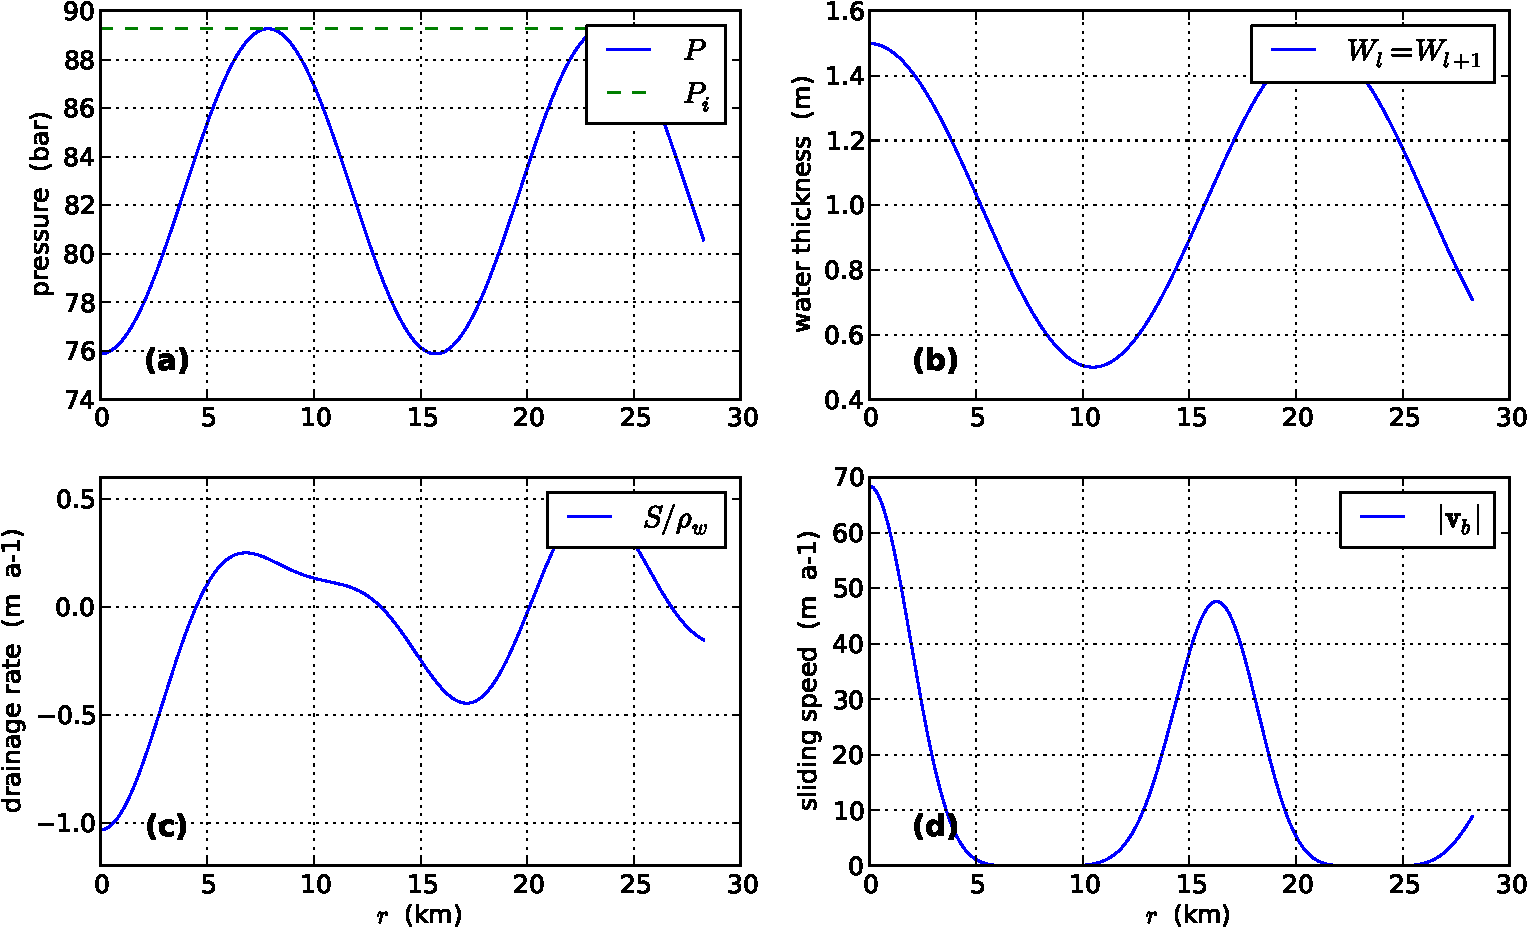
\includegraphics[width=6.2in,keepaspectratio=true]{figs/verifcase1}
\caption{Verification Case 1:  \textbf{(a)} Chosen water pressure $P(r)$, with constant overburden pressure $P_0$ for scale.  \textbf{(b)} Chosen water thickness $W^l(r)=W^{l+1}(r)$.  \textbf{(c)} Manufactured surface/englacial drainage $S(r)$ as a thickness rate.  \textbf{(d)} Manufactured sliding speed $|\bv_b(r)|$.}
\label{fig:verifcase1}
\end{figure}


\subsection*{Verification Case 2}  We define water thicknesses $W^{l+1}(r)$, $W^{l}(r)$ of somewhat different form from Case 1, and with time-dependent values, but so that $W^{l+1}(0) = W^{l}(0) = 0$ is a location of discontinuous gradient:
\begin{equation} \label{eq:manuWWtwo}
W^l(r) = \delta_0 r e^{-r/\alpha_0}, \qquad W^{l+1}(r) = \delta_0 r e^{-r/\alpha_1}.\end{equation}
See Figure \ref{fig:verifcase2}.

For the pressure, in this case we first define a nontrivial thickness profile appropriate to an ice sheet,
\begin{equation} \label{eq:profiletwo}
H(r) = \frac{H_0}{(1-n^{-1})^m} \left[q\left(\frac{r}{L_s}\right) - \frac{1}{n} + \left(1 - \frac{r}{L_s}\right)^q - \left(\frac{r}{L_s}\right)^q \right]^m
\end{equation}
where $m=n/(2n+2)$ and $q = (n+1)/n$ \citep[][subsection FIXME]{GreveBlatter2009}.  This profile has a zero-thickness margin at $r=L_s$, $H(L_s)=0$, while $H(0)=H_0$.  Thus the overburden pressure $P_o(r) = \rho_i g H(r)$ is non-constant and $P_o(L_s)=0$.  We also define a different pressure distribution from Case 1,
\begin{equation} \label{eq:manuPtwo}
P(r) = \frac{P_0}{3} \left(2\cos\left(2 \beta r\right) + 1\right),
\end{equation}
where $P_0 = 0.9 \rho_i g H_0$ and $\beta = \pi / (3 L_s)$.  Note that
\begin{equation*}
\nabla \cdot \left(W^{l+j} \nabla P\right) = - \frac{4}{3} \delta_0 P_0 \beta e^{-r/\alpha_j} \left(\left(2-\frac{r}{\alpha_j}\right)\sin(2\beta r) + 2 \beta r \cos(2 \beta r)\right).
\end{equation*}

Equation \eqref{eq:amountVERIF} then provides $S$,
\begin{align}
S &= \frac{\rho_w}{\Delta t} \left(W^{l+1}(r) - W^{l}(r)\right) \label{eq:Sveriftwo} \\ 
  &\qquad + \frac{4}{3} \rho_w c_0 \delta_0 P_0 \beta e^{-r/\alpha_1} \left[\left(2 - \frac{r}{\alpha_1}\right) \sin\left(2 \beta r\right) + 2 \beta r \cos\left(2 \beta r\right)\right], \notag
\end{align}
with $W^{l+1}(r)$ and $W^{l}(r)$ from \eqref{eq:manuWWtwo}.  Then equation \eqref{eq:pressureVERIF} provides the formula for the sliding:
\begin{align}
|\bv_b|(r) &= \frac{1}{\Cavit} \left[c_0 \nabla \cdot \left(W^l \nabla P\right) + \Creep A (P_o - P)^n W^l + \frac{S}{\rho_w}\right] \label{eq:slidingveriftwo}  \\
   &= - \frac{4 \pi c_0 P_0 \delta_0}{9 L_s \Cavit} e^{-r/\alpha_0} \left[\left(2 - \frac{r}{\alpha_0}\right) \sin\left(2 \beta r\right) + 2 \beta r \cos\left(2 \beta r\right)\right] \notag \\
   &\qquad + \frac{\Creep A}{\Cavit} \left(P_o(r) - P(r)\right)^n W^l(r) + \frac{S}{\rho_w \Cavit}, \notag
\end{align}
where $P_o(r) = \rho_i g H(r)$ uses equation \eqref{eq:profiletwo}, equation \eqref{eq:manuPtwo} provides $P(r)$, equation \eqref{eq:manuWWtwo} provides $W^l(r)$, and equation \eqref{eq:Sveriftwo} provides $S(r)$.  Again Table \ref{tab:verifconstants} gives values for constants needed in the construction of this Case 2 verification solution, while Figure \ref{fig:verifcase2} shows these radial functions.

\begin{figure}[ht]
\centering
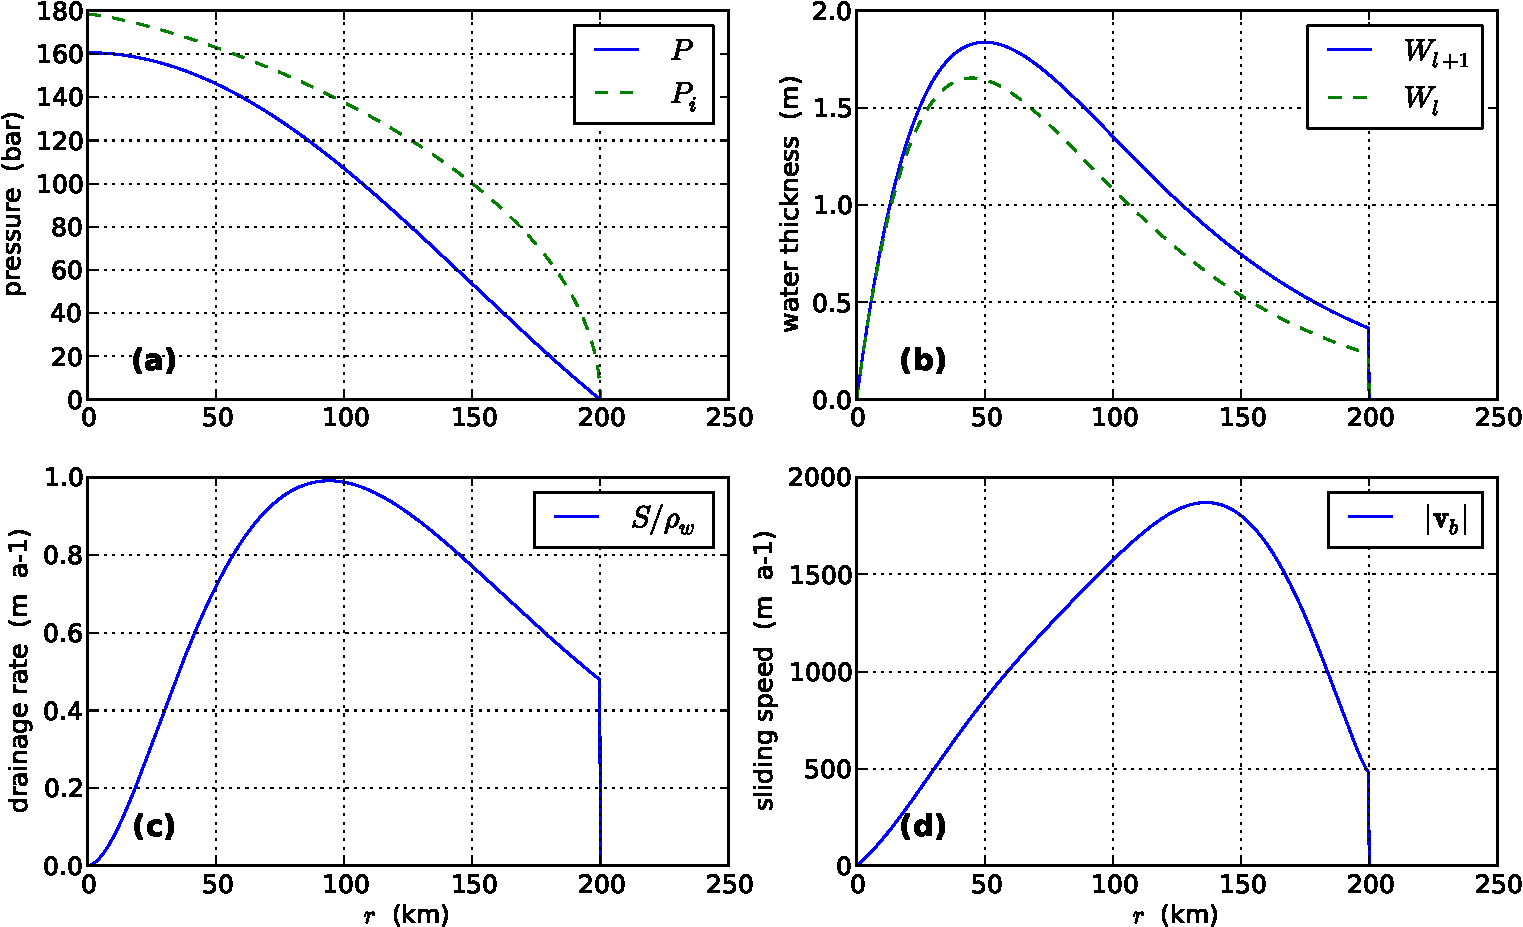
\includegraphics[width=6.2in,keepaspectratio=true]{figs/verifcase2}
\caption{Verification Case 2:  \textbf{(a)} Chosen water pressure $P(r)$ and overburden pressure $P_o(r) = \rho_i g H(r)$.  \textbf{(b)} Chosen initial water thickness $W^l(r)$ and final water thickness $W^{l+1}(r)$.  \textbf{(c)} Manufactured surface/englacial drainage $S(r)$ as a thickness rate.  \textbf{(d)} Manufactured sliding speed $|\bv_b(r)|$.}
\label{fig:verifcase2}
\end{figure}


\subsection*{Accuracy on verification tests}  The verification process itself starts by entering formulas for $S$ and $|\bv_b|$ from the above into a numerical program.  Also $W^l$ is entered as part of the data.  The program approximately solves PDEs \eqref{eq:pressureVERIF} and \eqref{eq:amountVERIF} for $P$ and $W^{l+1}$, respectively.  Boundary values for $P$ and $W^{l+1}$ are taken from the exact solutions when doing the numerical calculation.  Then the numerically computed values for $P$ and $W^{l+1}$ are compared to values from the formulas \eqref{eq:manuPone}/\eqref{eq:manuPtwo} and \eqref{eq:manuWWone}/\eqref{eq:manuWWtwo}, respectively.  The numerical computation is done on an $x,y$ cartesian grid, so verification will test the degree to which the computation has artifacts aligned to the grid.  This verification process is only a step in the process of correct implementation.  Numerical experiments and comparison to data (validation) follow verification.

Figure \ref{fig:convergecase1} shows results for Case 1.  Here the solutions for $\psi$ and $W^{l+1}$ are smooth all the way to the edge of the square computational domain $\left\{|x| \le 20 \text{ km}, \, |y| \le 20 \text{ km}\right\}$.  The decay of the error for $\psi$, as the square mesh size $\Delta x = \Delta y$ is reduced, shows that scheme \eqref{eq:Pfd} achieves its intended $O(\Delta x^2 + \Delta y^2)$ accuracy when solving equation \eqref{eq:pressureSEMI}.  The decay of the error for $W^{l+1}$ is much slower, first of all because the upwinding method \eqref{eq:Wfd} is only designed to achieve $O(\Delta x^1 + \Delta y^1)$ accuracy when solving equation \eqref{eq:amountSEMI}.  It is not clear why the observed decay of the error is slightly slower than that, but one reason may be that the function $\psi$ used in equation \eqref{eq:amountSEMI} is the computed result from using \eqref{eq:Pfd} to solve \eqref{eq:pressureSEMI}, and this numerically computed field is less smooth than the exact solution.  Probably because finite differences are used to evaluate the Jacobian in these results, the maximum error in $W^{l+1}$ from the finest grid $\Delta x = 62.5$ m is an ``outlier'', which is not included in computing the rate of decay.

\begin{figure}[ht]
\centering
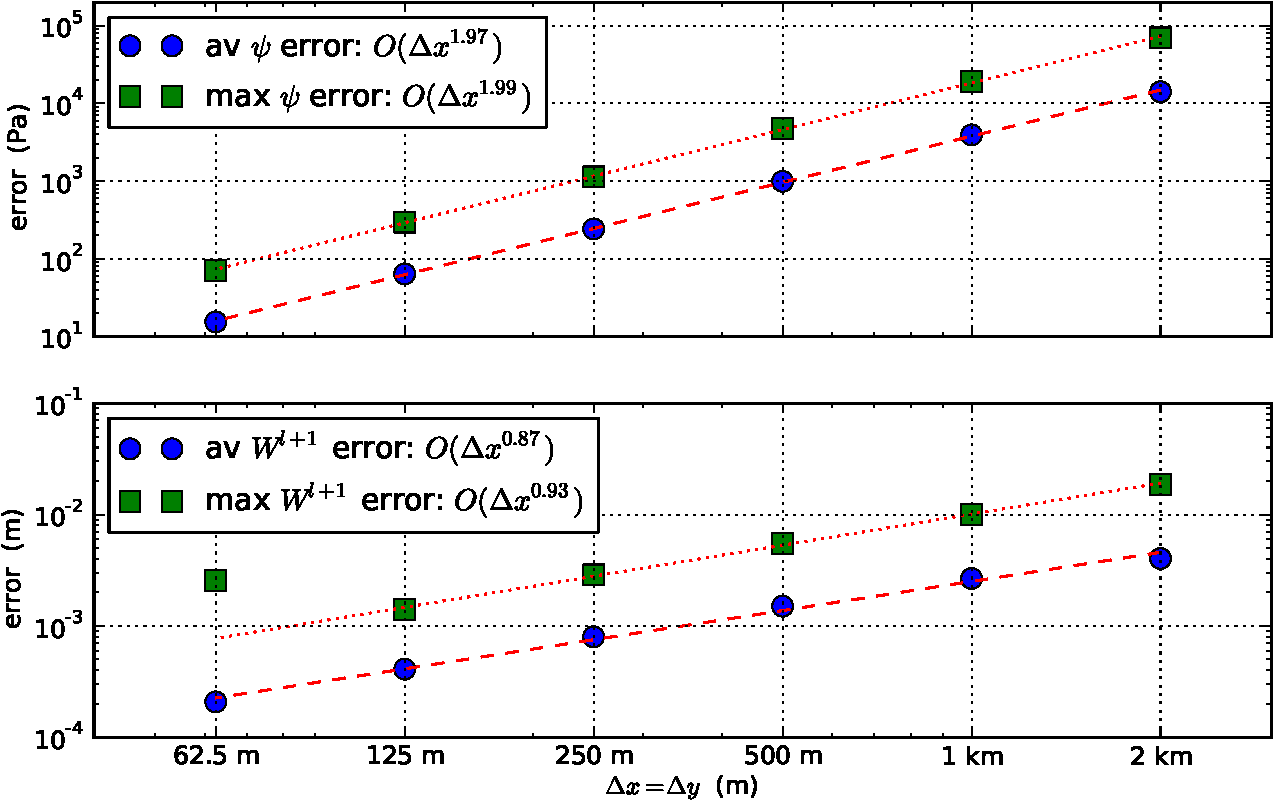
\includegraphics[width=5.5in,keepaspectratio=true]{figs/convergecase1}
\caption{Verification Case 1 results:  Measured average and maximum errors in hydraulic potential $\psi$ \textbf{(top)} and measured average and maximum errors in updated water thickness $W^{l+1}$ \textbf{(bottom)}.  Given rates of convergence are from linear regression of the error data to a power relation (i.e.~error $= C \Delta x^p$); see text.}
\label{fig:convergecase1}
\end{figure}

\subsection*{On computational speed}

\section{Results}


\section{Discussion}


\section{Conclusion}



\small
\bibliography{ice-bib}  % generally requires link to pism/doc/ice-bib.bib
\bibliographystyle{agu}

\appendix

\section{Boundary conditions from weak form of obstacle problem}  As do \cite{Schoofetal2012} and \cite{Hewittetal2012}, we can describe the formulation of the pressure problem as a double obstacle problem.  This helps understand the boundary conditions for the pressure problem, and the regularity (smoothness) of its solution.

Let $\Omega$ be the area (open subset of the plane) covered by grounded ice sheet.  This set is not assumed to be connected.  The boundary $\partial\Omega$ includes land margin where the water pressure is atmospheric, where we set atmospheric (zero) pressure, and also marine grounding lines where the effective pressure is zero.  At such marine grounding lines the subglacial water pressure has boundary value $P= \rho_i g H = -\rho_{sw} g b$, where $\rho_{sw}$ is the density of sea water and zero is the elevation of sea level.  Define
	$$\partial \Omega_a = \left\{(x,y)\in \partial \Omega  \, \big| \, b(x,y) \ge 0\right\}, \qquad \partial \Omega_m = \left\{(x,y)\in \partial \Omega  \, \big| \, b(x,y) < 0\right\}$$
for the subaerial and marine parts of the ice margin.

Define $\psi_b = \rho_w g b$, the hydraulic potential corresponding to zero water pressure, and $\psi_i = \rho_i g H + \psi_b$, the hydraulic potential corresponding to overburden pressure.  We now want to capture the idea that the hydraulic potential $\psi$ which solves the problem is between $\psi_b$ and $\psi_i$, and that it has the correct boundary values on the subaerial and marine parts of the margin.  We are also concerned that $\psi$ be the kind of function that could solve an elliptic PDE.  Recall that $W^{1,2}(\Omega)$ denotes the space of functions on $\Omega$ whose gradients are square-integrable \citep{Evans}.  We will assume that $\psi_b, \psi_i \in W^{1,2}(\Omega)$, and we will assume that $\partial \Omega$ is not too irregular (e.g.~it is Lipshitz).

Let
	$$W^{1,2}_D(\Omega) = \left\{\phi \in W^{1,2}(\Omega) \, \big| \quad \phi(\partial \Omega_a) = \psi_b, \quad \phi(\partial \Omega_m) = \psi_i\right\},$$
where ``$D$'' stands for ``satisfies the Dirichlet conditions.''  Let
\begin{equation}\label{eq:admissible}
	\mathcal{K} = \left\{\phi \in W^{1,2}_D(\Omega) \, \big| \, \psi_b \le \phi \le \psi_i\right\}
\end{equation}
define the convex set of admissible functions for the hydraulic potential.  ``Admissible'' means that the function both has the correct boundary values and satisfies inequalities \eqref{eq:psibounds}.  Figure \ref{fig:boundary} shows these admissibility conditions.

\begin{figure}[ht]
\centering
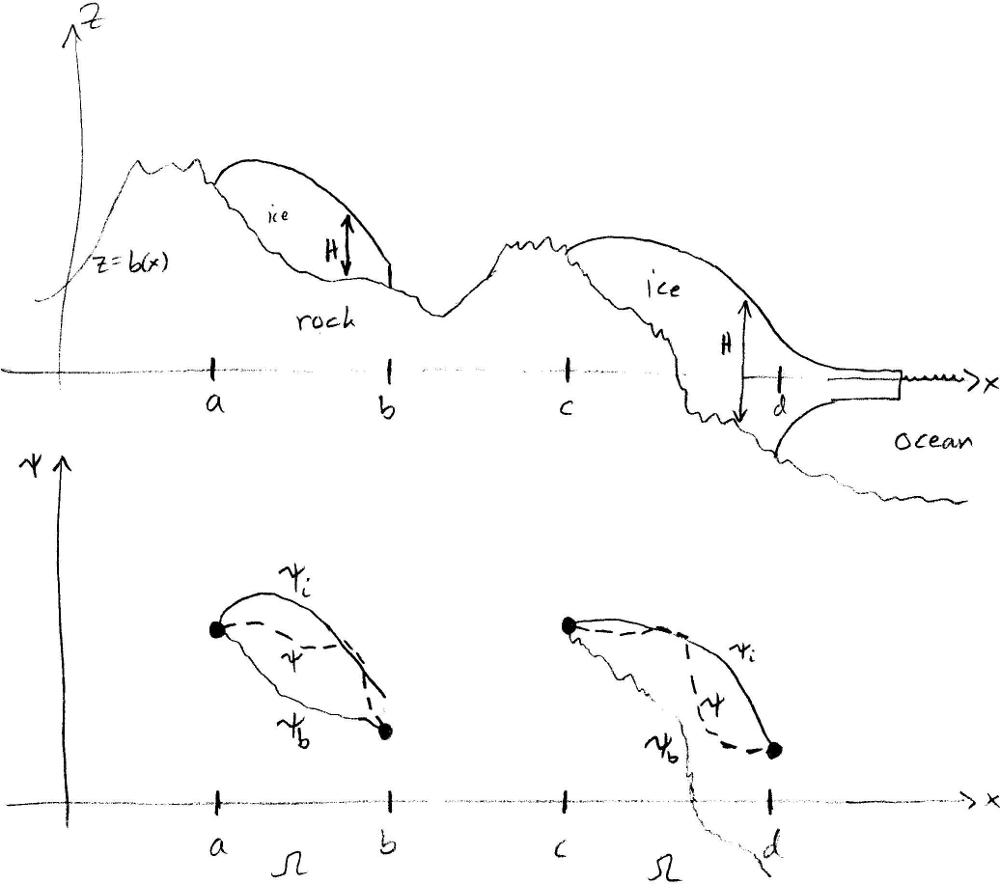
\includegraphics[width=4.0in,keepaspectratio=true]{figs/boundary_cartoon}
\caption{A sketch of what boundary conditions apply to $\psi$ in a one-dimensional case, showing geometry \textbf{(top)} and hydraulic potential for subglacial water \textbf{(bottom)}.  At \textbf{a}, \textbf{b}, and \textbf{c} we have the subaerial condition $\psi=\psi_b$.  At \textbf{d} we have the marine condition $\psi=\psi_i$.  At all points where the ice is present, the constraints $\psi_b\le \psi \le \psi_i$ must apply.}
\label{fig:boundary}
\end{figure}

For $\phi \in \mathcal{K}$, define the functional
\begin{equation}\label{eq:functionalJ}
   J[\phi] = \int_\Omega \frac{c_0}{2} W^l |\nabla \phi|^2 + \frac{\Creep A }{n+1} W^l \left(\psi_i - \phi\right)^{n+1} + \mathcal{M}_0 \phi,
\end{equation}
where $\mathcal{M}_0 = \Cavit |\bv_b| + L^{-1} (-\tau_b \cdot \bv_b + G) - \rho_w^{-1} S$ is a combination of melting and opening which we suppose\footnote{``Suppose'' is appropriate.  In fact the velocity $\bv_b$ and the basal shear stress $\tau_b$ should, at least ideally and possibly in practice, be determined by simultaneous equations with the basal water pressure.  This certainly applies to time-steps which are of significant magnitude so that changes in contact area with bed protrusions have occurred along with (presumably even faster) changes in water pressure.} is determined independently of the solution of the pressure problem, and where the integration is over map-plane area (i.e.~with the usual area element $dx\,dy$).  We assume that $W^l$ and $\mathcal{M}_0$  are bounded (in $L^\infty(\Omega)$).  Note that a function in $W^{1,2}(\Omega)$ is in $L^{n+1}(\Omega)$ for $n<\infty$ so $J[\phi]$ is therefore finite \citep{Evans}.

A minimum of functional $J$ is our proposed solution to the pressure problem (when $\Cmelt=0$).  In fact, suppose $\psi$ minimizes $J$.  If $\phi \in \mathcal{K}$ is another admissible function, then $\psi + \epsilon (\phi - \psi) \in \mathcal{K}$ for any $0\le \epsilon \le 1$ because $\mathcal{K}$ is convex.  Then we have
\begin{align*}
0 &\le J[\psi+\epsilon(\phi-\psi)] - J[\psi] \\
   &= \int_\Omega \frac{c_0}{2} W^l \left[2 \epsilon \nabla \psi \cdot \nabla (\phi-\psi) + \epsilon^2 |\nabla (\phi-\psi)|^2\right] \\
   &\qquad\qquad + \frac{\Creep A }{n+1} W^l \left[\left(\psi_i - \psi - \epsilon(\phi-\psi)\right)^{n+1} - \left(\psi_i - \psi\right)^{n+1}\right] + \mathcal{M}_0 \epsilon (\phi - \psi)  \\
   &= \epsilon \left[\int_\Omega c_0 W^l \nabla \psi \cdot \nabla (\phi-\psi) - \Creep A W^l (\psi_i - \psi)^n (\phi-\psi) + \mathcal{M}_0(\phi - \psi)\right] \, + O(\epsilon^2)
\end{align*}
by the binomial expansion.  Thereby the minimization statement about $\psi$ becomes a statement about the derivative of the functional,
	$$0 \le \lim_{\eps\to 0^+} \frac{J[\psi+\epsilon(\phi-\psi)] - J[\psi]}{\epsilon}.$$
That is, the minimizer $\psi \in \mathcal{K}$ of the functional $J$ also has the property
\begin{equation}\label{eq:vi}
\int_\Omega c_0 W^l \nabla \psi \cdot \nabla (\phi-\psi) - \Creep A W^l (\psi_i - \psi)^n (\phi-\psi) + \mathcal{M}_0(\phi - \psi)\, \ge\, 0 \qquad \text{for all}\,\phi\in\mathcal{K}.
\end{equation}
This last statement is a \emph{variational inequality}.

We claim that if a solution $\psi$ of equation \eqref{eq:pressureSEMI} is admissible ($\psi \in \mathcal{K}$) and sufficiently smooth then it satisfies \eqref{eq:vi}.  ``Sufficiently smooth'' means that we can integrate by parts; when we do that the boundary term is zero, because $\phi$ and $\psi$ have the same Dirichlet boundary conditions, and we get
	$$\int_\Omega - c_0 \nabla \cdot \left(W^l \nabla \psi\right) \,(\phi-\psi) - \Creep A W^l (\psi_i - \psi)^n (\phi-\psi) + \mathcal{M}_0(\phi - \psi)\, \ge\, 0$$
for all $\phi\in\mathcal{K}$.  But now $(\phi - \psi)$ factors, and, because $\psi$ satisfies $- c_0 \nabla \cdot \left(W^l \nabla \psi\right) - \Creep A W^l (\psi_i - \psi)^n + \mathcal{M}_0=0$, the left side of \eqref{eq:vi} is identically zero and the inequality is satisfied.  Conversely, if $\psi$ solves \eqref{eq:vi} then, on subsets of $\Omega$ where the potential is not ``up against'' one of the constraining inequalities, that is, where $\psi_b < \psi < \psi_i$, then one can show by introducing $\phi=\psi+\nu$ where $\nu$ is a small-amplitude, smooth function with compact support on $\psi_b < \psi < \psi_i$, that the PDE \eqref{eq:pressureSEMI} is satisfied by $\psi$ \citep[page 469]{Evans}.

The above computations following the definition of the functional \eqref{eq:functionalJ} are standard parts of the calculus of variations.  They show why minimizing $J$ is  closely-related to solving equation \eqref{eq:pressureSEMI}.  Irregular functions, however, including those which are sometimes against the constraints (i.e.~either $\psi=\psi_b$ or $\psi=\psi_i$), or which do not have $C^2$ smoothness for other reasons, can minimize $J$ even when they do not satisfy a PDE like  \eqref{eq:pressureSEMI} in the ``strong'' sense.  In fact, the existence of a minimizer of $J$ is clear from quite general considerations \cite[chapter 8]{Evans}, at least where $W^l>0$, but, because of the creep-closure term in particular, the uniqueness of the minimizer is far from clear and may not be true.  Nonetheless, more is known about the well-posedness of the weak problem ``minimize $J$ subject to boundary conditions and constraints'' than about the corresponding strong problem ``solve \eqref{eq:pressureSEMI} subject to boundary conditions and constraints.''

Furthermore we can learn from thinking about minimizing $J$.   Consider cases where there is no water ($W^l=0$) or very small amounts of water ($W^l \ll 1$ m).  In such cases the functional $J$ is dominated by the last term:
	$$W^l \approx 0 \qquad \implies \qquad J[\phi] \approx \int_\Omega \mathcal{M}_0 \phi.$$
In such areas where there is no/small water $W^l \approx 0$ we can make $J$ small by making the input $\phi$ bigger or smaller according to the sign of $\mathcal{M}_0$.  If $\mathcal{M}_0$ is dominated by englacial drainage $\mathcal{M}_0=-S/\rho_w$, for example, we expect that the minimizer is as big as possible: $\psi=\psi_i$.  That is, we see from the minimization framework that the pressure will tend to its limits:
	$$W^l \approx 0 \qquad \implies \qquad \begin{cases} \psi=\psi_i & \text{where } \mathcal{M}_0 < 0, \\ \psi=\psi_b & \text{where } \mathcal{M}_0 > 0.\end{cases}$$
These discussions are significantly motivated by the problem of setting the pressure in areas where there is a transition from frozen bed (thus $W^l=0$) to more significant water.  In any case, PDE \eqref{eq:pressureSEMI} does not supply a value in no-water areas, so the minimization framework has assisted us.
% FIXME:  further thought on this may be rewarded by additional understanding ...


\section{Why we are not doing the same thing as Schoof et al.}  Note that \cite{Schoofetal2012} recently came out.  That paper---part I in particular---is clearly comparable to our intent.  Here are the differences I see:
\begin{enumerate}
\item Ours is 2D, parallel, and part of a comprehensive ice flow model.
\item Ours assumes $W=Y$, which is ``$h_w=h$'' in his terms, because we do no care about, or allow, under pressure.
\item Compared to equation (2.12) in \cite{Schoofetal2012}, our equation for pressure \eqref{eq:pressurePDE} uses $\alpha = 1$ and $\beta=2$ to have less nonlinearity.
\item We do consider (i.e.~allow) wall melt in our distributed model.  \cite{Schoofetal2012} does not consider it, and \cite{Hewittetal2012} only considers it in channels.  We expose ourselves to the \cite{Walder1982} instability this way, but we believe that it is stopped/limited by the \cite{CreytsSchoof2009} bed protrusions argument.
\item Our $\Delta t$ comes from the ice flow model.  It may be huge compared to the natural timescale, essentially the CFL time for equation \eqref{eq:amountPDE}.  So we use an implicit method, instead of the explicit method in \cite{Schoofetal2012} and \cite{Hewittetal2012}, to update water amount.  Essentially we may get a sequence of steady states for \eqref{eq:amountPDE}, but that is what we want.
\end{enumerate}

\end{document}
